\chapter{Validation}
\label{chap:Validation}

Samples:
\begin{itemize}
    \item \textcolor{green}{Standard BNB $\electron \pi^+$}
    \item \textcolor{green}{Standard BNB $\gamma \pi^+$}
    \item \textcolor{green}{Standard BNB cheating $\electron \pi^+$}
    \item \textcolor{orange}{SCE cheating cathode BNB $\electron \pi^+$}
    \item \textcolor{orange}{SCE cheating anode BNB $\electron \pi^+$}
    \item \textcolor{green}{XZ plane cheating $\electron \pi^+$ - may need to remake with uniform angular dist.}
    \item \textcolor{green}{YZ plane cheating $\electron \pi^+$}
    \item \textcolor{red}{Standard BNB with lower thresholding $\electron \pi^+$}
    \item \textcolor{red}{Some low energy sample}
\end{itemize}

\begin{figure}
    \centering
    \fbox{Fractional resolution using $\electron \pi^+$ BNB vertex sample for plane 0}
    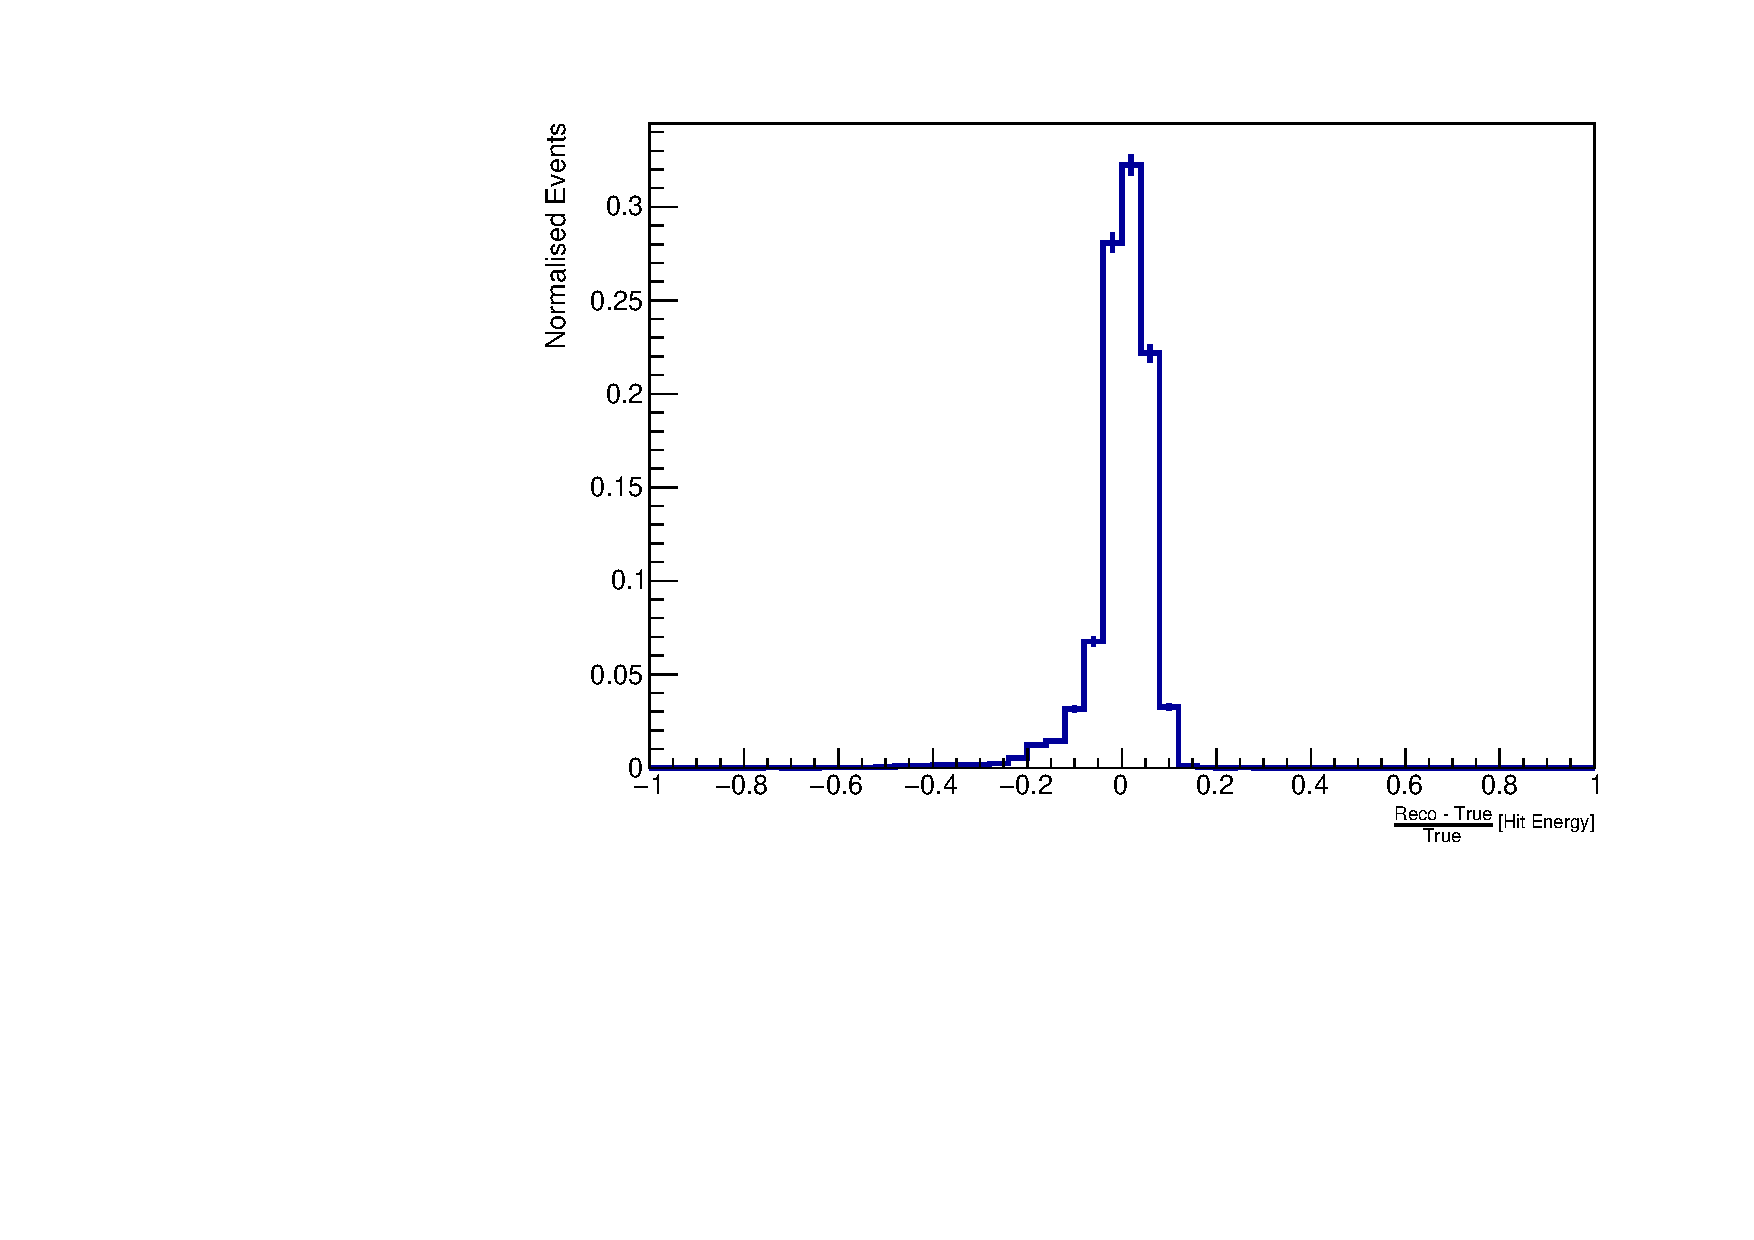
\includegraphics[width = \largefigwidth]{Figures/fractional_res_standard_electron_vertex_plane0.pdf}
    \caption{Fractional resolution of the shower energy from an $\electron \pi^+$ vertex sample. Reconstruction performed from the hits collected by plane 0.}
    \label{fig:my_label}
\end{figure}

\begin{figure}
    \centering
    \fbox{Fractional resolution using $\electron \pi^+$ BNB vertex sample for plane 1}
    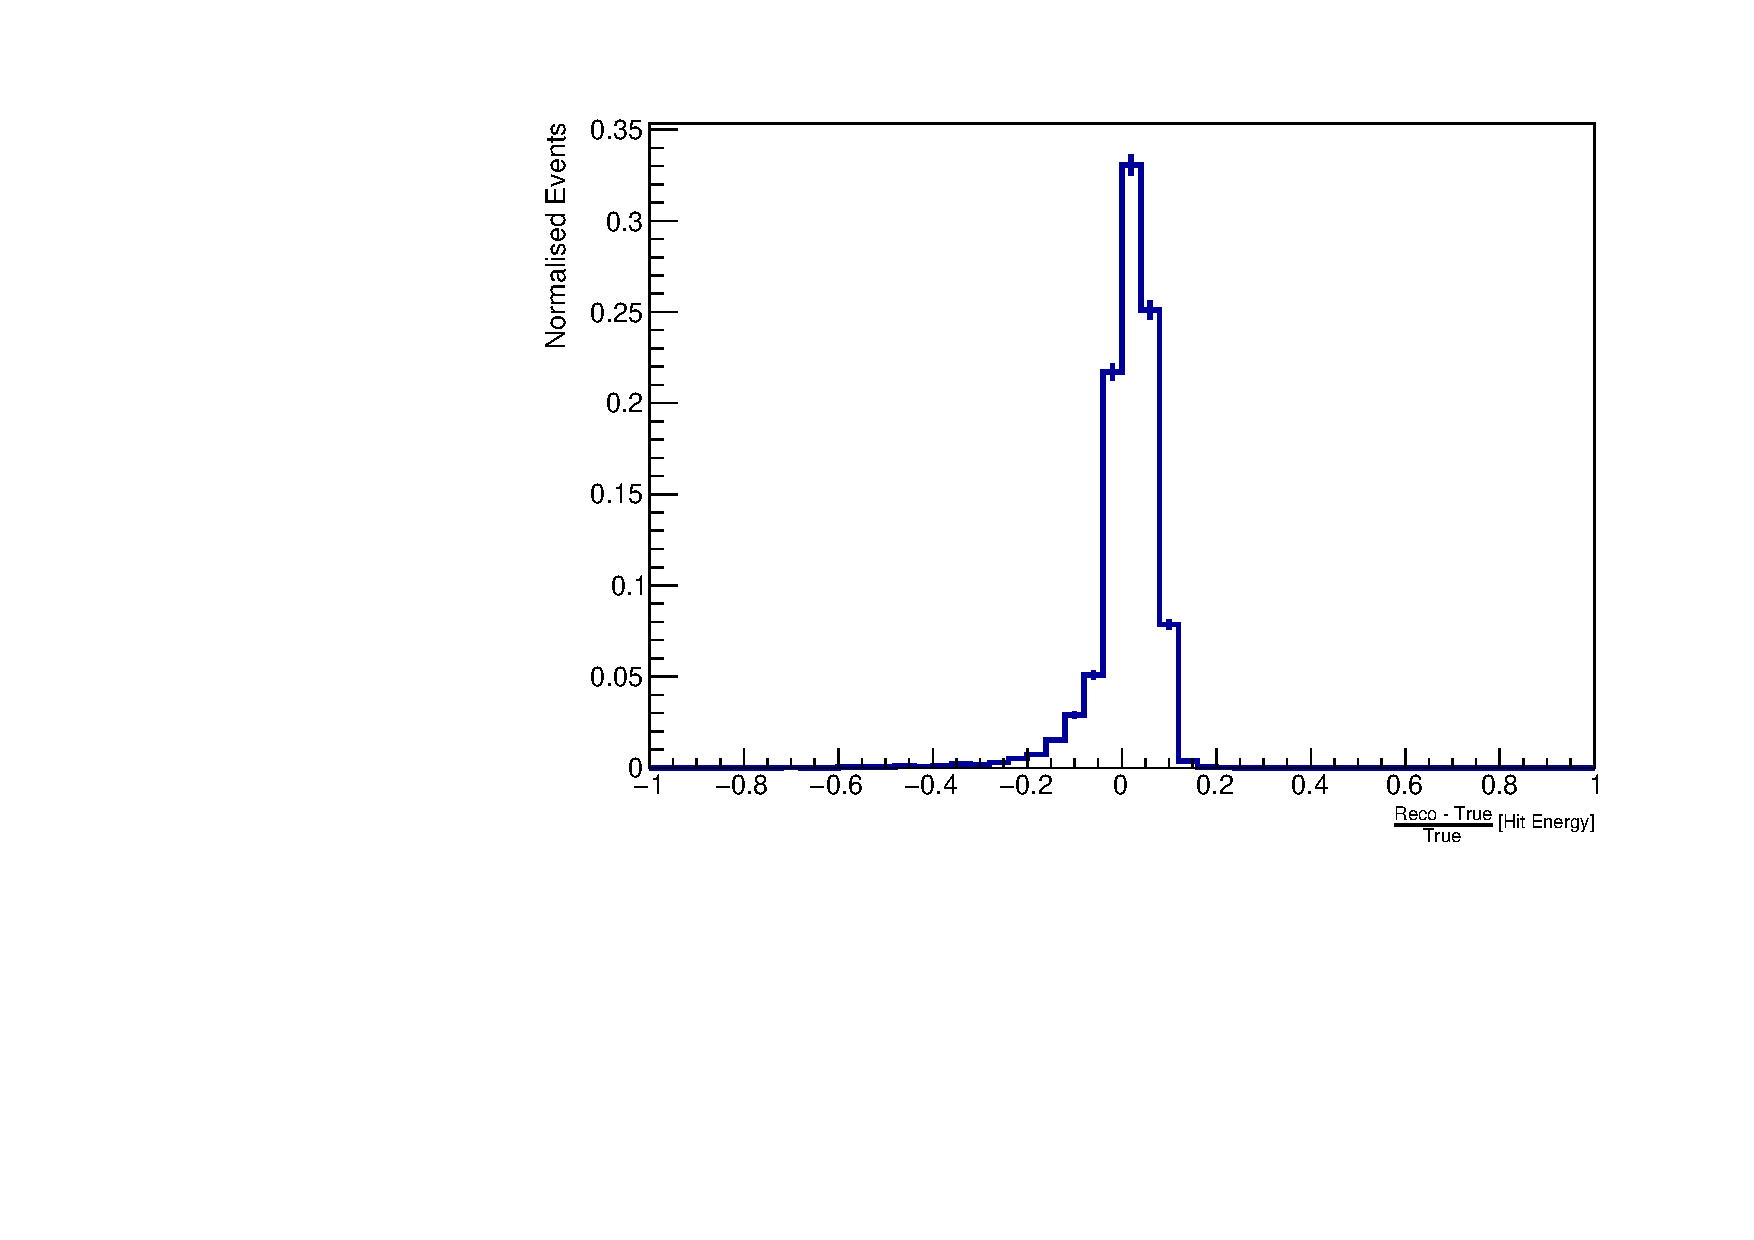
\includegraphics[width = \largefigwidth]{Figures/fractional_res_standard_electron_vertex_plane1.pdf}
    \caption{Fractional resolution of the shower energy from an $\electron \pi^+$ vertex sample. Reconstruction performed from the hits collected by plane 1.}
    \label{fig:my_label}
\end{figure}

\begin{figure}
    \centering
    \fbox{Fractional resolution using $\electron \pi^+$ BNB vertex sample for plane 2}
    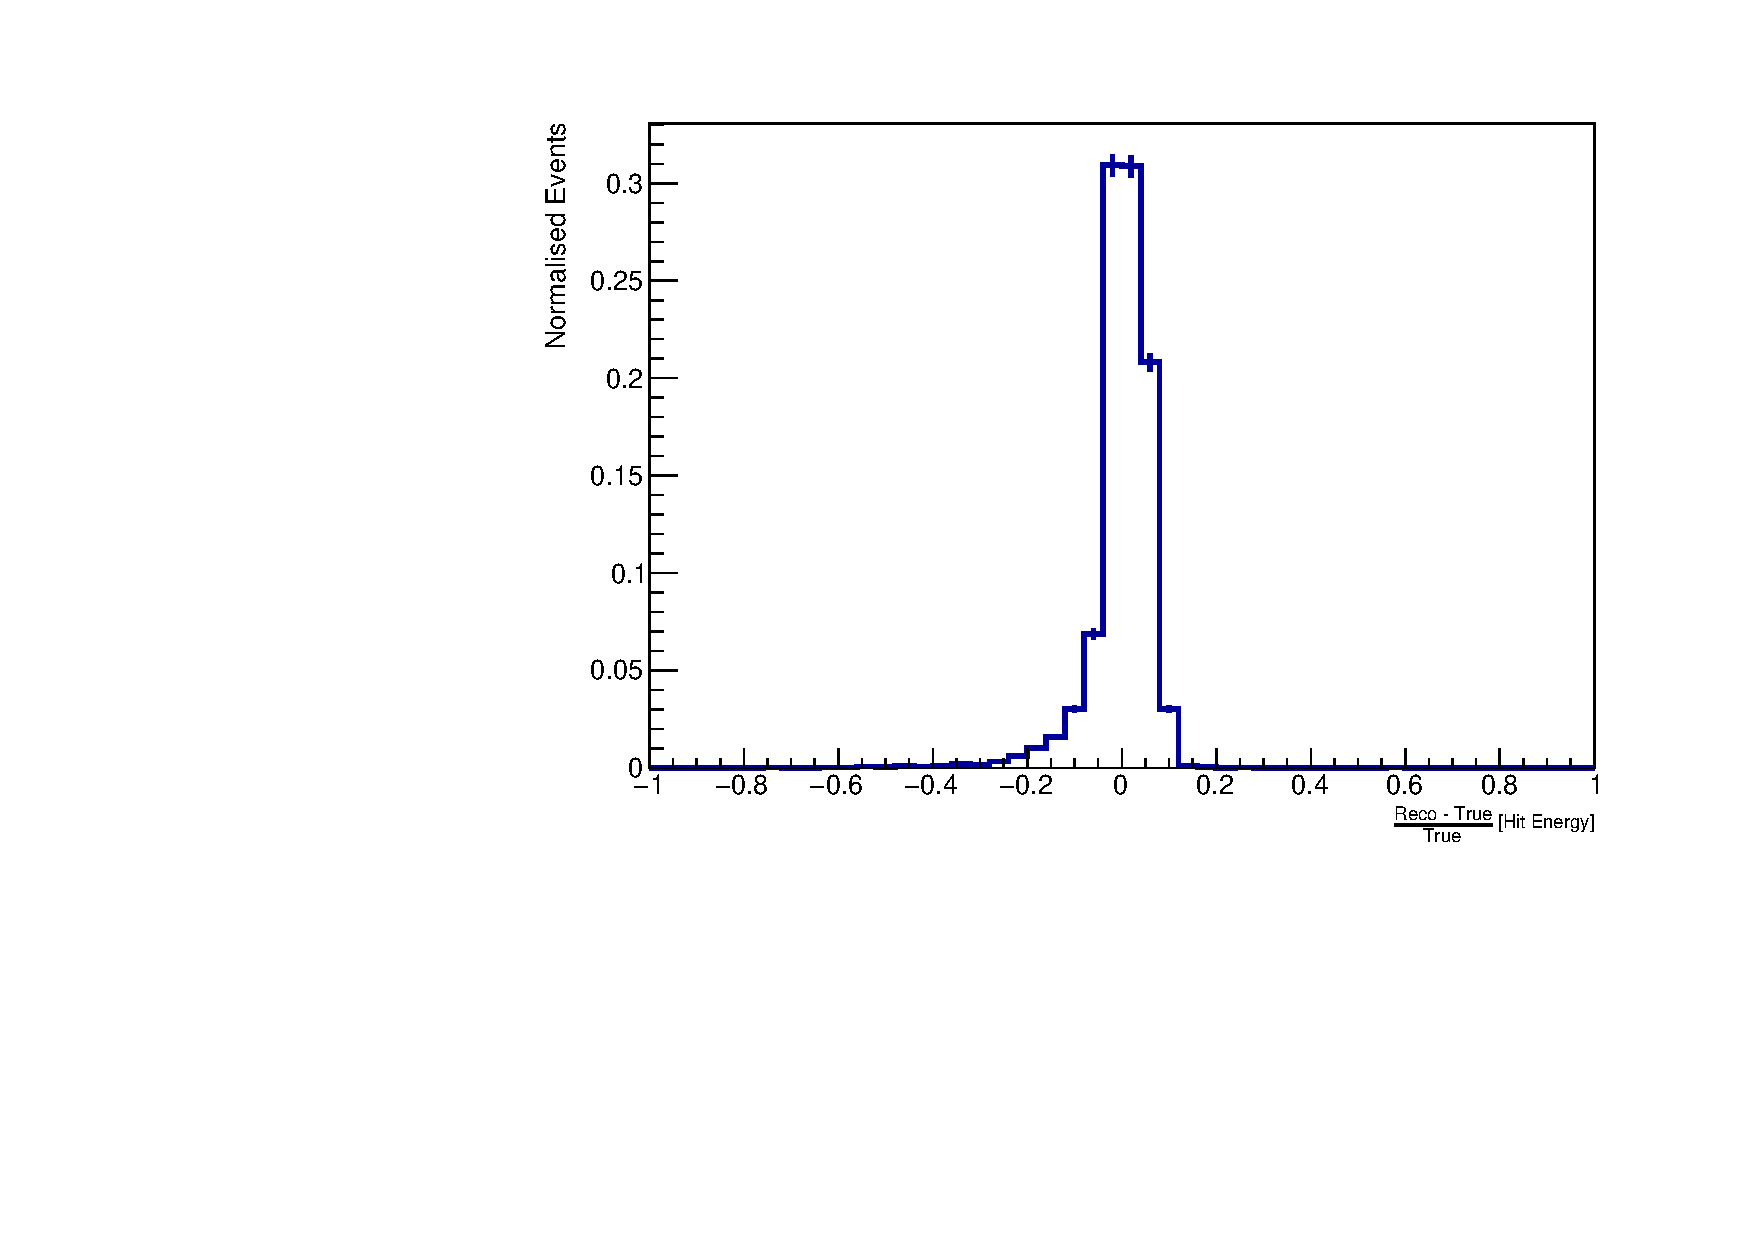
\includegraphics[width = \largefigwidth]{Figures/fractional_res_standard_electron_vertex_plane2.pdf}
    \caption{Fractional resolution of the shower energy from an $\electron \pi^+$ vertex sample. Reconstruction performed from the hits collected by plane 2.}
    \label{fig:my_label}
\end{figure}

\begin{figure}
    \centering
    \fbox{Fractional resolution using $\electron \pi^+$ BNB vertex sample for the best plane}
    \caption{Caption}
    \label{fig:my_label}
\end{figure}

\begin{figure}
    \centering
    \fbox{Fractional resolution using $\electron \pi^+$ BNB vertex sample with cheated pattern recognition.}
    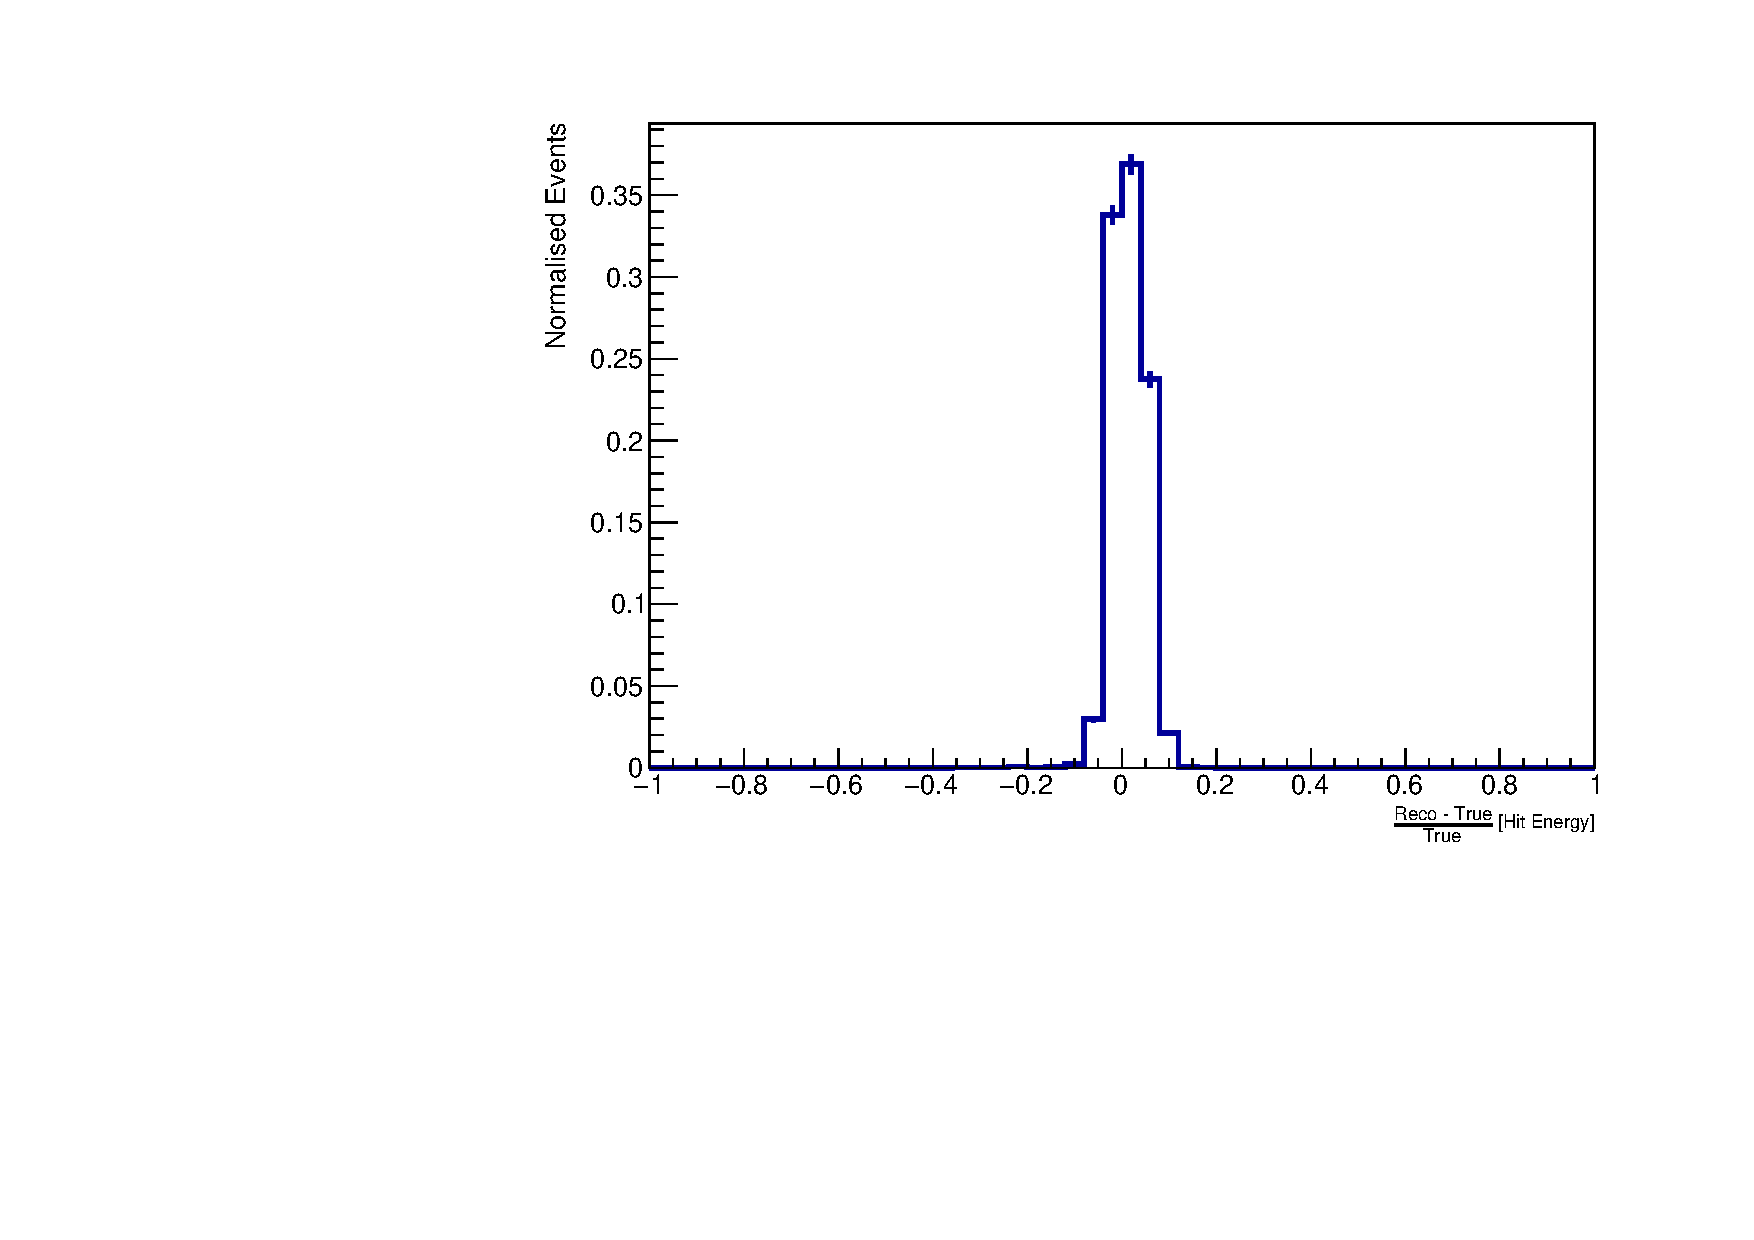
\includegraphics[width = \largefigwidth]{Figures/fractional_res_standard_cheating_electron_vertex_plane2.pdf}
    \caption{Fractional resolution of the shower energy from an $\electron \pi^+$ vertex sample with cheated pattern recognition. Reconstruction performed from the hits collected by plane 2.}
    \label{fig:my_label}
\end{figure}

\begin{figure}
    \centering
    \fbox{Fractional resolution using $\gamma \pi^+$ BNB vertex sample}
    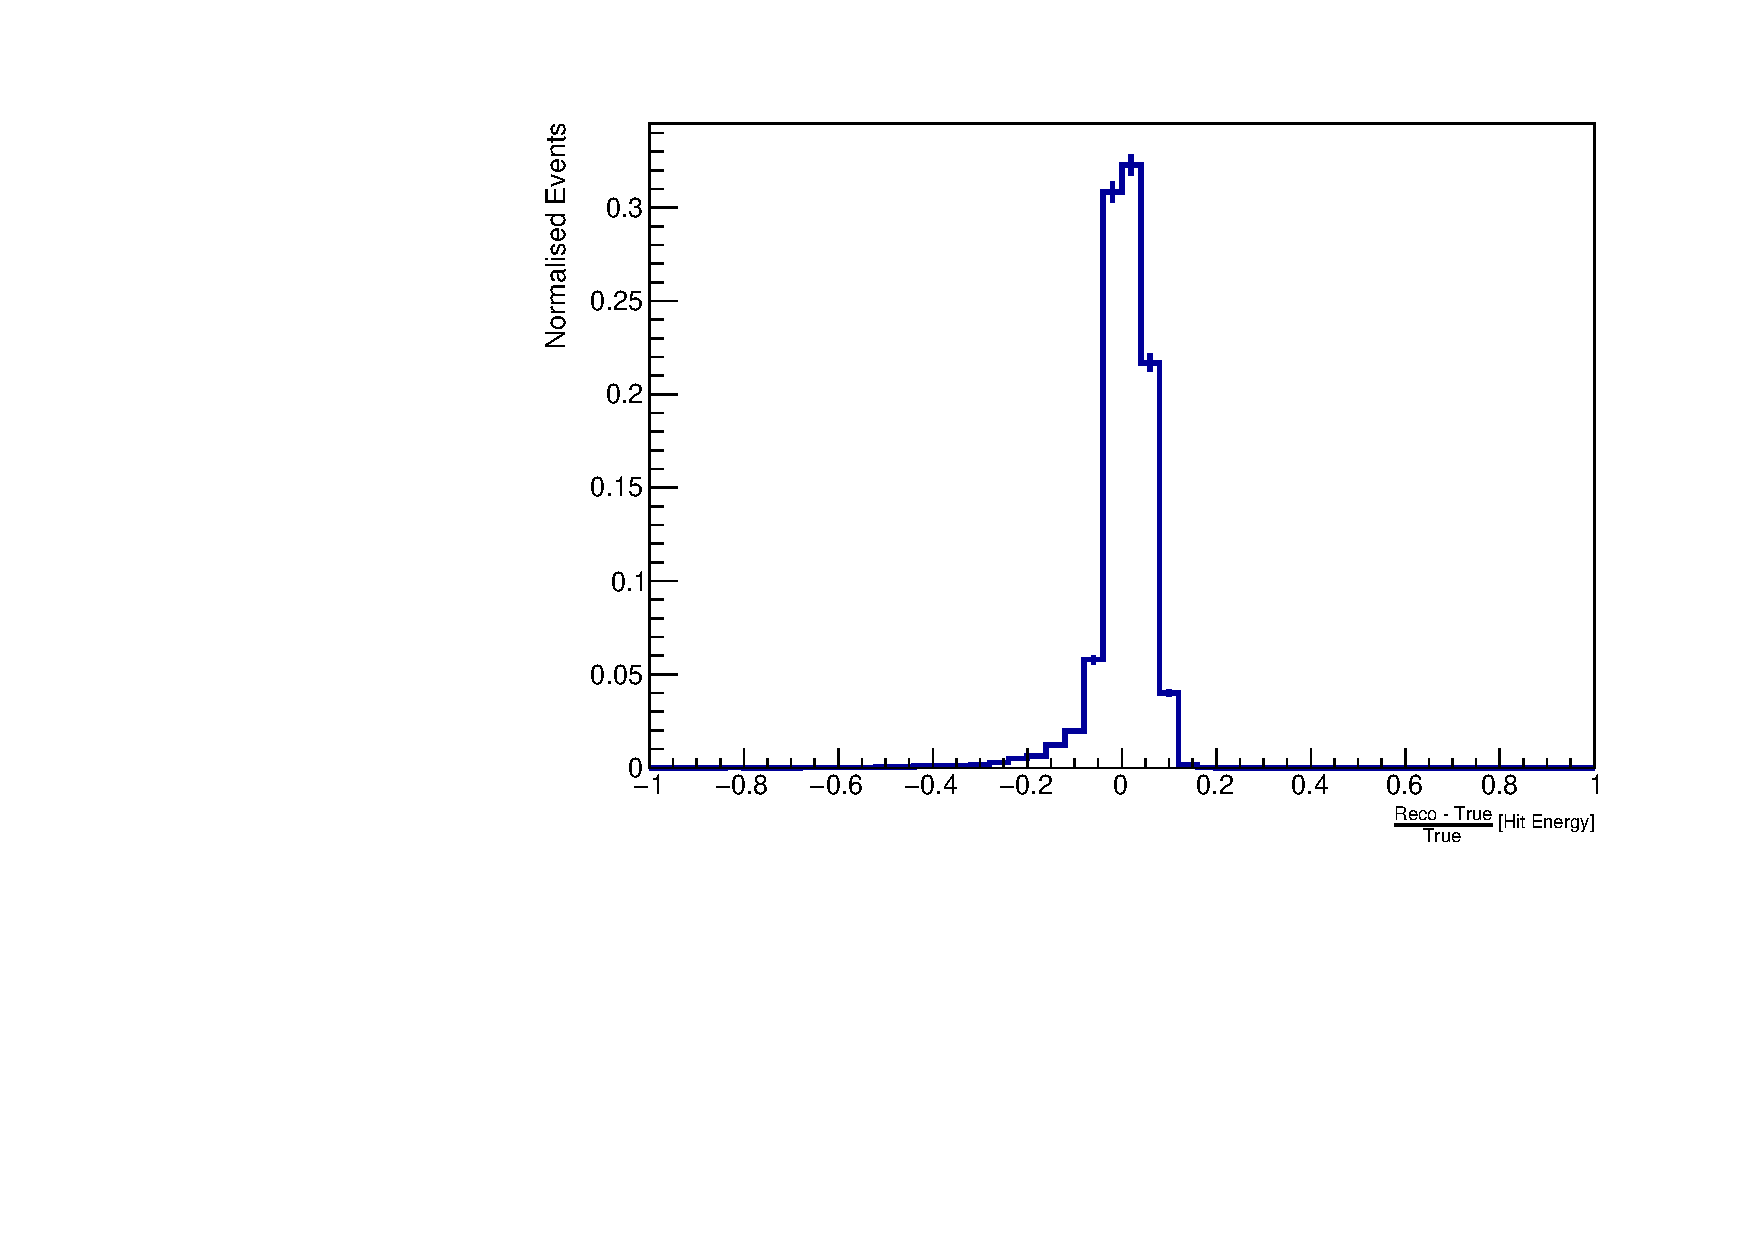
\includegraphics[width = \largefigwidth]{Figures/fractional_res_standard_gamma_vertex_plane2.pdf}
    \caption{Fractional resolution of the shower energy using a $\gamma \pi^+$ vertex sample. Reconstruction performed from the hits collected by plane 2.}
    \label{fig:my_label}
\end{figure}

\begin{figure}
    \centering
    \fbox{
    \begin{minipage}{0.8\textwidth}
    Space Charge validation. Fractional resolution plot for cathode sample w.o. SCE, w. SCE but no correction and w. SCE + correction. Plus include ratio plot.
    Use cheated pattern recognition. \newline
    
    \end{minipage}
    }
    \caption{Caption}
    \label{fig:my_label}
\end{figure}

\begin{figure}
    \centering
    \fbox{
    \begin{minipage}{0.8\textwidth}
    Space Charge validation. Fractional resolution plot for anode sample w.o. SCE, w. SCE but no correction and w. SCE + correction. Plus include ratio plot.
    Use cheated pattern recognition. \newline
    
    \end{minipage}
    }
    \caption{Caption}
    \label{fig:my_label}
\end{figure}












